\documentclass[]{book}
\usepackage{lmodern}
\usepackage{amssymb,amsmath}
\usepackage{ifxetex,ifluatex}
\usepackage{fixltx2e} % provides \textsubscript
\ifnum 0\ifxetex 1\fi\ifluatex 1\fi=0 % if pdftex
  \usepackage[T1]{fontenc}
  \usepackage[utf8]{inputenc}
\else % if luatex or xelatex
  \ifxetex
    \usepackage{mathspec}
  \else
    \usepackage{fontspec}
  \fi
  \defaultfontfeatures{Ligatures=TeX,Scale=MatchLowercase}
\fi
% use upquote if available, for straight quotes in verbatim environments
\IfFileExists{upquote.sty}{\usepackage{upquote}}{}
% use microtype if available
\IfFileExists{microtype.sty}{%
\usepackage{microtype}
\UseMicrotypeSet[protrusion]{basicmath} % disable protrusion for tt fonts
}{}
\usepackage[margin=1in]{geometry}
\usepackage{hyperref}
\hypersetup{unicode=true,
            pdftitle={An Introduction to Statistical Programming Methods with R},
            pdfauthor={Matthew Beckman, Stéphane Guerrier, Justin Lee \& Roberto Molinari},
            pdfborder={0 0 0},
            breaklinks=true}
\urlstyle{same}  % don't use monospace font for urls
\usepackage{natbib}
\bibliographystyle{apalike}
\usepackage{color}
\usepackage{fancyvrb}
\newcommand{\VerbBar}{|}
\newcommand{\VERB}{\Verb[commandchars=\\\{\}]}
\DefineVerbatimEnvironment{Highlighting}{Verbatim}{commandchars=\\\{\}}
% Add ',fontsize=\small' for more characters per line
\usepackage{framed}
\definecolor{shadecolor}{RGB}{248,248,248}
\newenvironment{Shaded}{\begin{snugshade}}{\end{snugshade}}
\newcommand{\KeywordTok}[1]{\textcolor[rgb]{0.13,0.29,0.53}{\textbf{{#1}}}}
\newcommand{\DataTypeTok}[1]{\textcolor[rgb]{0.13,0.29,0.53}{{#1}}}
\newcommand{\DecValTok}[1]{\textcolor[rgb]{0.00,0.00,0.81}{{#1}}}
\newcommand{\BaseNTok}[1]{\textcolor[rgb]{0.00,0.00,0.81}{{#1}}}
\newcommand{\FloatTok}[1]{\textcolor[rgb]{0.00,0.00,0.81}{{#1}}}
\newcommand{\ConstantTok}[1]{\textcolor[rgb]{0.00,0.00,0.00}{{#1}}}
\newcommand{\CharTok}[1]{\textcolor[rgb]{0.31,0.60,0.02}{{#1}}}
\newcommand{\SpecialCharTok}[1]{\textcolor[rgb]{0.00,0.00,0.00}{{#1}}}
\newcommand{\StringTok}[1]{\textcolor[rgb]{0.31,0.60,0.02}{{#1}}}
\newcommand{\VerbatimStringTok}[1]{\textcolor[rgb]{0.31,0.60,0.02}{{#1}}}
\newcommand{\SpecialStringTok}[1]{\textcolor[rgb]{0.31,0.60,0.02}{{#1}}}
\newcommand{\ImportTok}[1]{{#1}}
\newcommand{\CommentTok}[1]{\textcolor[rgb]{0.56,0.35,0.01}{\textit{{#1}}}}
\newcommand{\DocumentationTok}[1]{\textcolor[rgb]{0.56,0.35,0.01}{\textbf{\textit{{#1}}}}}
\newcommand{\AnnotationTok}[1]{\textcolor[rgb]{0.56,0.35,0.01}{\textbf{\textit{{#1}}}}}
\newcommand{\CommentVarTok}[1]{\textcolor[rgb]{0.56,0.35,0.01}{\textbf{\textit{{#1}}}}}
\newcommand{\OtherTok}[1]{\textcolor[rgb]{0.56,0.35,0.01}{{#1}}}
\newcommand{\FunctionTok}[1]{\textcolor[rgb]{0.00,0.00,0.00}{{#1}}}
\newcommand{\VariableTok}[1]{\textcolor[rgb]{0.00,0.00,0.00}{{#1}}}
\newcommand{\ControlFlowTok}[1]{\textcolor[rgb]{0.13,0.29,0.53}{\textbf{{#1}}}}
\newcommand{\OperatorTok}[1]{\textcolor[rgb]{0.81,0.36,0.00}{\textbf{{#1}}}}
\newcommand{\BuiltInTok}[1]{{#1}}
\newcommand{\ExtensionTok}[1]{{#1}}
\newcommand{\PreprocessorTok}[1]{\textcolor[rgb]{0.56,0.35,0.01}{\textit{{#1}}}}
\newcommand{\AttributeTok}[1]{\textcolor[rgb]{0.77,0.63,0.00}{{#1}}}
\newcommand{\RegionMarkerTok}[1]{{#1}}
\newcommand{\InformationTok}[1]{\textcolor[rgb]{0.56,0.35,0.01}{\textbf{\textit{{#1}}}}}
\newcommand{\WarningTok}[1]{\textcolor[rgb]{0.56,0.35,0.01}{\textbf{\textit{{#1}}}}}
\newcommand{\AlertTok}[1]{\textcolor[rgb]{0.94,0.16,0.16}{{#1}}}
\newcommand{\ErrorTok}[1]{\textcolor[rgb]{0.64,0.00,0.00}{\textbf{{#1}}}}
\newcommand{\NormalTok}[1]{{#1}}
\usepackage{longtable,booktabs}
\usepackage{graphicx,grffile}
\makeatletter
\def\maxwidth{\ifdim\Gin@nat@width>\linewidth\linewidth\else\Gin@nat@width\fi}
\def\maxheight{\ifdim\Gin@nat@height>\textheight\textheight\else\Gin@nat@height\fi}
\makeatother
% Scale images if necessary, so that they will not overflow the page
% margins by default, and it is still possible to overwrite the defaults
% using explicit options in \includegraphics[width, height, ...]{}
\setkeys{Gin}{width=\maxwidth,height=\maxheight,keepaspectratio}
\IfFileExists{parskip.sty}{%
\usepackage{parskip}
}{% else
\setlength{\parindent}{0pt}
\setlength{\parskip}{6pt plus 2pt minus 1pt}
}
\setlength{\emergencystretch}{3em}  % prevent overfull lines
\providecommand{\tightlist}{%
  \setlength{\itemsep}{0pt}\setlength{\parskip}{0pt}}
\setcounter{secnumdepth}{5}
% Redefines (sub)paragraphs to behave more like sections
\ifx\paragraph\undefined\else
\let\oldparagraph\paragraph
\renewcommand{\paragraph}[1]{\oldparagraph{#1}\mbox{}}
\fi
\ifx\subparagraph\undefined\else
\let\oldsubparagraph\subparagraph
\renewcommand{\subparagraph}[1]{\oldsubparagraph{#1}\mbox{}}
\fi

%%% Use protect on footnotes to avoid problems with footnotes in titles
\let\rmarkdownfootnote\footnote%
\def\footnote{\protect\rmarkdownfootnote}

%%% Change title format to be more compact
\usepackage{titling}

% Create subtitle command for use in maketitle
\newcommand{\subtitle}[1]{
  \posttitle{
    \begin{center}\large#1\end{center}
    }
}

\setlength{\droptitle}{-2em}
  \title{An Introduction to Statistical Programming Methods with R}
  \pretitle{\vspace{\droptitle}\centering\huge}
  \posttitle{\par}
  \author{Matthew Beckman, Stéphane Guerrier, Justin Lee \& Roberto Molinari}
  \preauthor{\centering\large\emph}
  \postauthor{\par}
  \predate{\centering\large\emph}
  \postdate{\par}
  \date{2017-08-20}

\usepackage{booktabs}
\usepackage{amsthm}
\makeatletter
\def\thm@space@setup{%
  \thm@preskip=8pt plus 2pt minus 4pt
  \thm@postskip=\thm@preskip
}
\makeatother

\usepackage{amsthm}
\newtheorem{theorem}{Theorem}[chapter]
\newtheorem{lemma}{Lemma}[chapter]
\theoremstyle{definition}
\newtheorem{definition}{Definition}[chapter]
\newtheorem{corollary}{Corollary}[chapter]
\newtheorem{proposition}{Proposition}[chapter]
\theoremstyle{definition}
\newtheorem{example}{Example}[chapter]
\theoremstyle{remark}
\newtheorem*{remark}{Remark}
\let\BeginKnitrBlock\begin \let\EndKnitrBlock\end
\begin{document}
\maketitle

{
\setcounter{tocdepth}{1}
\tableofcontents
}
\chapter{Introduction}\label{introduction}

This book is currently under development and has been designed as a
support for students who are following (or are interested in) courses
that provide the basic knowledge to master ``statistical programming''
with R. By the latter we mean that area of computer programming which
focuses on the implementation of methods that not only manage data but
also extract meaningful information from it. The importance of this area
of research comes from the increased collection of data from different
sources such as academic research, public institutions and private
companies that has required a corresponding increase in data management
and analysis tools. Consequently, the need to develop applications and
methods that are able to deliver these tools has led to a surge in the
demand for expertise not only in computer programming but also in
statistical and numerical analysis. Indeed, while it is essential to
master the basics of programming to build the necessary software, it is
now also paramount to understand the programming tools that can
effectively respond to the need of finding, extracting, and analyzing
the information to achieve the required goals.

Within the above framework, the statistical software \texttt{R} has seen
a rise in use due to its flexibility as an efficient language that
builds a bridge between software development and data analysis. There
are of course many other programming languages that have different
advantages over \texttt{R} but, as you will see, one strength of
\texttt{R} is the facility to develop and quickly adapt to the different
needs coming from the data management and analysis community while at
the same time making use of other languages in order to deliver
computationally efficient solutions (as well as other interesting
features described below). This book intends to present the basic tools
to statistical programming and software development using the wide
variety of tools made available through \texttt{R}, from method-specific
packages to version control programs. The general goals of the book are
therefore the following:

\begin{itemize}
\tightlist
\item
  understand data structures in order to appropriately manage data,
  computer memory and computations;
\item
  manipulate data structures through controls, instructions, and
  tailored functions in order to achieve a desired output;
\item
  create new software tools (packages and web applications) that
  accommodate a previously unmet need;
\item
  learn how to manage software development via version control tools
  (e.g., GitHub) and create documentation for this software (with
  embedded code) to allow others to make use of the software.
\end{itemize}

All these goals are common to any basic programming course, however all
these will be heavily focused on the use and development of statistical
tools. In fact, as highlighted earlier, it has become increasingly
important to include statistical methodologies within the programming
framework thereby allowing software to not only manage data efficiently
but also to extract and analyse data in an appropriate manner while
doing so. The rest of this introductory chapter will present the R
software by explaining why it is used for this book and describing the
basic notations and tools that need to be known in order to better grasp
its contents.

\BeginKnitrBlock{rmdimportant}
This document is \textbf{under development} and it is therefore
preferable to always access the text online to be sure you are using the
most up-to-date version. Due to its current development, you may
encounter errors ranging from broken code to typos or poorly explained
topics. If you do, please let us know! Simply add an issue to the GitHub
repository used for this document (which can be accessed here
\url{https://github.com/SMAC-Group/ds/issues}) and we will make the
changes as soon as possible. In addition, if you know RMarkdown and are
familiar with GitHub, make a pull request and fix an issue yourself,
otherwise, if you're not familiar with these tools, they will be
explained later on in the book itself.
\EndKnitrBlock{rmdimportant}

\section{\texorpdfstring{\texttt{R} and
\texttt{RStudio}}{R and RStudio}}\label{r-and-rstudio}

The statistical computing language \texttt{R} has become commonplace for
many applications in industry, government, and academia. Having started
as an open-source language to make available different statistics and
analytical tools to researchers and the public, it steadily developed
into one of the major software languages which not only allows to
develop up-to-date, sound, and flexible analytical tools, but also to
include these tools within a framework which is well-integrated with
other important programming languages, communication, and
version-control features. The latter is also possible thanks to the
development of the \texttt{RStudio} interface which provides a pleasant
and functional user-interface for \texttt{R} as well as an efficient
Integrated Development Environment (IDE) in which different programming
languages, web-applications and other important tools are available to
the user. In order to illustrate the relationship between R \& RStudio
in statistical programming, one might think of a car analogy in which R
would be like the engine and RStudio might be like leather seats. R is
doing the work (for the most part), and RStudio generally is making you
more comfortable while you use R.

\subsection{\texorpdfstring{Why \texttt{R}?}{Why R?}}\label{why-r}

There are many reasons to use \texttt{R}. Two compelling reasons are
that R is both free as in ``free pizza'', and free as in ``free
speech''). Free--like ``free pizza''--means that there is never a need
to pay for any part of the R software, or contributed packages
(i.e.~add-on modules). Free--like ``free speech''--means that there are
very few restrictions on how R can be used or barriers to those who
would like to contribute packages (i.e.~add-on modules).

The fact that is a free and open-source software which \emph{per se}
does not necessarily imply that it is a good software (although it is
also that). The reason why this is an important feature consists in the
fact that the results of any code or program developed in the \texttt{R}
environment can easily be replicated therefore ensuring accessibility
and transparency for the general user. More importantly however, this
replicability of results is also accompanied by a wide variety of
packages that are made available through the \texttt{R} environment in
which users can find a diversity of codes, functions and features that
are designed to tackle a large amount of programming and analytical
tasks. Moreover, these packages are relatively simple to create and are
extremely useful for code-sharing purposes since they enclose the codes,
functions and external dependencies that allow anyone to install any of
these features all at once in easy and efficient manner.

In addition to its accessibility and code-sharing features, \texttt{R}
has acquired visibility and importance mainly due to the cutting-edge
tools that it makes available to the general user. Indeed, a growing
area of research both in academia and in industry is Statistics and
Machine Learning through which it is possible to find, extract and make
an efficient use of the increasing amount of data and information being
collected. All the latest methods and approaches going from data-mining
techniques to predictive analysis are available in \texttt{R} and, due
to its nature, all future methods and approaches will be made available
to all users through \texttt{R}. For this reason, any individual,
company or organization has a keen interest in acquiring and developing
expertise in \texttt{R} since it makes available the most appropriate
tools for any data-based analysis and decision-making process.

Like any other software, there are of course some drawbacks with using
\texttt{R}. First, the presence of an extended amount of
user-contributed packages can make its usage and bug-reporting
problematic. Although this does not represent a major problem since many
forums exist and solutions are usually quickly fixed, there can be many
issues concerning package updates or deletions that can create problems
for other existing packages that depend on them. This is fairly rare,
but there can consequently be problems in the use of packages that
become obsolete and need to be fixed due to dependency issues. Another
drawback consists in the extensive use of computer memory that
\texttt{R} entails through its commands which generally give little
relevance to this issue. However, many different solutions are being
developed which deal with this problem along with the increased memory
made available by current operating systems.

In the perspective of improving the usage of computer memory, \texttt{R}
has been developing efficient and ``seemless'' connections with
high-performance languages which allow functions and packages to make
use of them thereby greatly lightening and accelerating computations
made through \texttt{R}. An important example of this is given by the
connections made available to the \texttt{C++} language. In this book we
will discuss the connections with this language that are particularly
well implemented, but other high-performance languages can be used such
as \texttt{C} and \texttt{FORTRAN}.

\subsection{\texorpdfstring{Getting started with
\texttt{R}}{Getting started with R}}\label{getting-started-with-r}

As mentioned earlier, \texttt{R} can be thought of as a programming
language as well as a software environment for statistical programming.
Since it is a free and open-source software, all you will need to do is
to download it from the following link:

\begin{itemize}
\tightlist
\item
  \href{https://cran.r-project.org/}{\texttt{R}}
\end{itemize}

Once you've downloaded and installed \texttt{R} on your computer you
will be able to start using the programming language and packages that
the \texttt{R} environment provides. Nevertheless, to make full use of
the latest developments and features of this software, in this book we
recommend using the IDE called \texttt{RStudio} which can be downloaded
from the following link:

\begin{itemize}
\tightlist
\item
  \href{https://www.rstudio.com/}{RStudio}
\end{itemize}

\BeginKnitrBlock{rmdimportant}
You cannot use \texttt{RStudio} without having installed \texttt{R} on
your computer.
\EndKnitrBlock{rmdimportant}

\subsection{About RStudio}\label{about-rstudio}

\texttt{RStudio} is a customizable IDE for the \texttt{R} enviornment
where the user can have easy access to plots, data, help, files, objects
and many other features that are useful to work efficiently with
\texttt{R}. For the most part, \texttt{RStudio} provides everything the
\texttt{R} user will need in a self-contained, and well-organized
environment. Moreover, it is possible to create ``projects'' in which it
is possible to create a dedicated environment space for sets of specific
functions and files aimed to deal with various tasks.

\textbf{Rob} what about a video here to introduce RStudio???

In addition, \texttt{RStudio} provides embedded functionality to utilize
collaborative version-control software including GitHub \& Subversion as
well as a set of powerful tools to save and communicate results (whether
they be simulations, data analysis, or presenting and making available a
new package to other users). Some examples of these tools are
\texttt{Rmarkdown} which can be used respectively to integrate written
narrative with embedded \texttt{R} code and other content, as well as
and \texttt{Shiny\ Web\ Apps} which can provide an interactive
user-friendly interface that permits a user to actively engage with a
wide variety of tools built in \texttt{R} without the need to encounter
raw \texttt{R} code. GitHub and \texttt{Rmarkdown} will be the object of
a more in-depth description in the first chapters of this book in order
to provide the reader with the version-control and annotation tools that
can be useful for the following chapters of this book.

\subsection{Conventions}\label{conventions}

Throughout this book, \texttt{R} code will be typeset using a
\texttt{monospace} font which is syntax highlighted. For example:

\begin{Shaded}
\begin{Highlighting}[]
\NormalTok{a =}\StringTok{ }\NormalTok{pi}
\NormalTok{b =}\StringTok{ }\FloatTok{0.5}
\KeywordTok{sin}\NormalTok{(a*b)}
\end{Highlighting}
\end{Shaded}

Similarly, \texttt{R} output lines (that usally appear in your Console)
will begin with \texttt{\#\#} and will not be syntax highlighted. The
output of the above example is the following:

\begin{verbatim}
## [1] 1
\end{verbatim}

Aside from \texttt{R} code and its outputs, this book will also insert
some boxes that will draw the reader's attention to important, curious,
or otherwise informative details. An example of these boxes was seen at
the beginning of this introduction where an important aspect was pointed
out to the reader regarding the ``under construction'' nature of this
book. Therefore the following boxes and symbols can be used to represent
information of different nature:

\BeginKnitrBlock{rmdimportant}
This is an important piece of information.
\EndKnitrBlock{rmdimportant}

\BeginKnitrBlock{rmdnote}
This is some additional information that could be useful to the reader.
\EndKnitrBlock{rmdnote}

\BeginKnitrBlock{rmdcaution}
This is something that the reader should pay caution to but should not
create major problems if not considered.
\EndKnitrBlock{rmdcaution}

\BeginKnitrBlock{rmdwarning}
This is a warning which should be heeded by the reader to avoid problems
of different nature.
\EndKnitrBlock{rmdwarning}

\BeginKnitrBlock{rmdtip}
This is a tip for the reader when following or developing something
based on this book.
\EndKnitrBlock{rmdtip}

\subsection{Simple calculations}\label{simple-calculations}

A basic aspect to underline about the \texttt{R} environment is that it
serves as an advanced calculator which therefore allows also for simple
calculations. In the table below we show a few examples of such
calculations where the first column gives a mathematical expression
(calculation), the second gives the equivalent of this expression in
\texttt{R} and finally in the third column we can find the result that
is output from \texttt{R}.

\begin{longtable}[]{@{}lll@{}}
\toprule
Math. & R & Result\tabularnewline
\midrule
\endhead
2+2 & \texttt{2+2} & \texttt{4}\tabularnewline
\(\frac{4}{2}\) & \texttt{4/2} & \texttt{2}\tabularnewline
\(3 \cdot 2^{-0.8}\) & \texttt{3*2\^{}(-0.8)} &
\texttt{1.723048}\tabularnewline
\(\sqrt{2}\) & \texttt{sqrt(2)} & \texttt{1.414214}\tabularnewline
\(\pi\) & \texttt{pi} & \texttt{3.141593}\tabularnewline
\(\ln(2)\) & \texttt{log(2)} & \texttt{0.6931472}\tabularnewline
\(\log_{3}(9)\) & \texttt{log(9,\ base\ =\ 3)} &
\texttt{2}\tabularnewline
\(e^{1.1}\) & \texttt{exp(1.1)} & \texttt{3.004166}\tabularnewline
\(\cos(\sqrt{0.9})\) & \texttt{cos(sqrt(0.9))} &
\texttt{0.5827536}\tabularnewline
\bottomrule
\end{longtable}

\subsection{Getting help}\label{getting-help}

In the previous section we presented some examples on how \texttt{R} can
be used as a calculator and we have already seen several functions such
as \texttt{sqrt()} or \texttt{log()}. To obtain documentation about a
function in \texttt{R}, simply put a question mark in front of the
function name (or just type \texttt{help()} around the function name),
or use the search bar on the ``Help'' tab in your RStudio window, and
its documentation will be displayed. For example, if you are interested
in learning about the function \texttt{log()} you could simply type:

\begin{Shaded}
\begin{Highlighting}[]
\NormalTok{?log}
\end{Highlighting}
\end{Shaded}

which will display something similar to:

\begin{figure}[htbp]
\centering
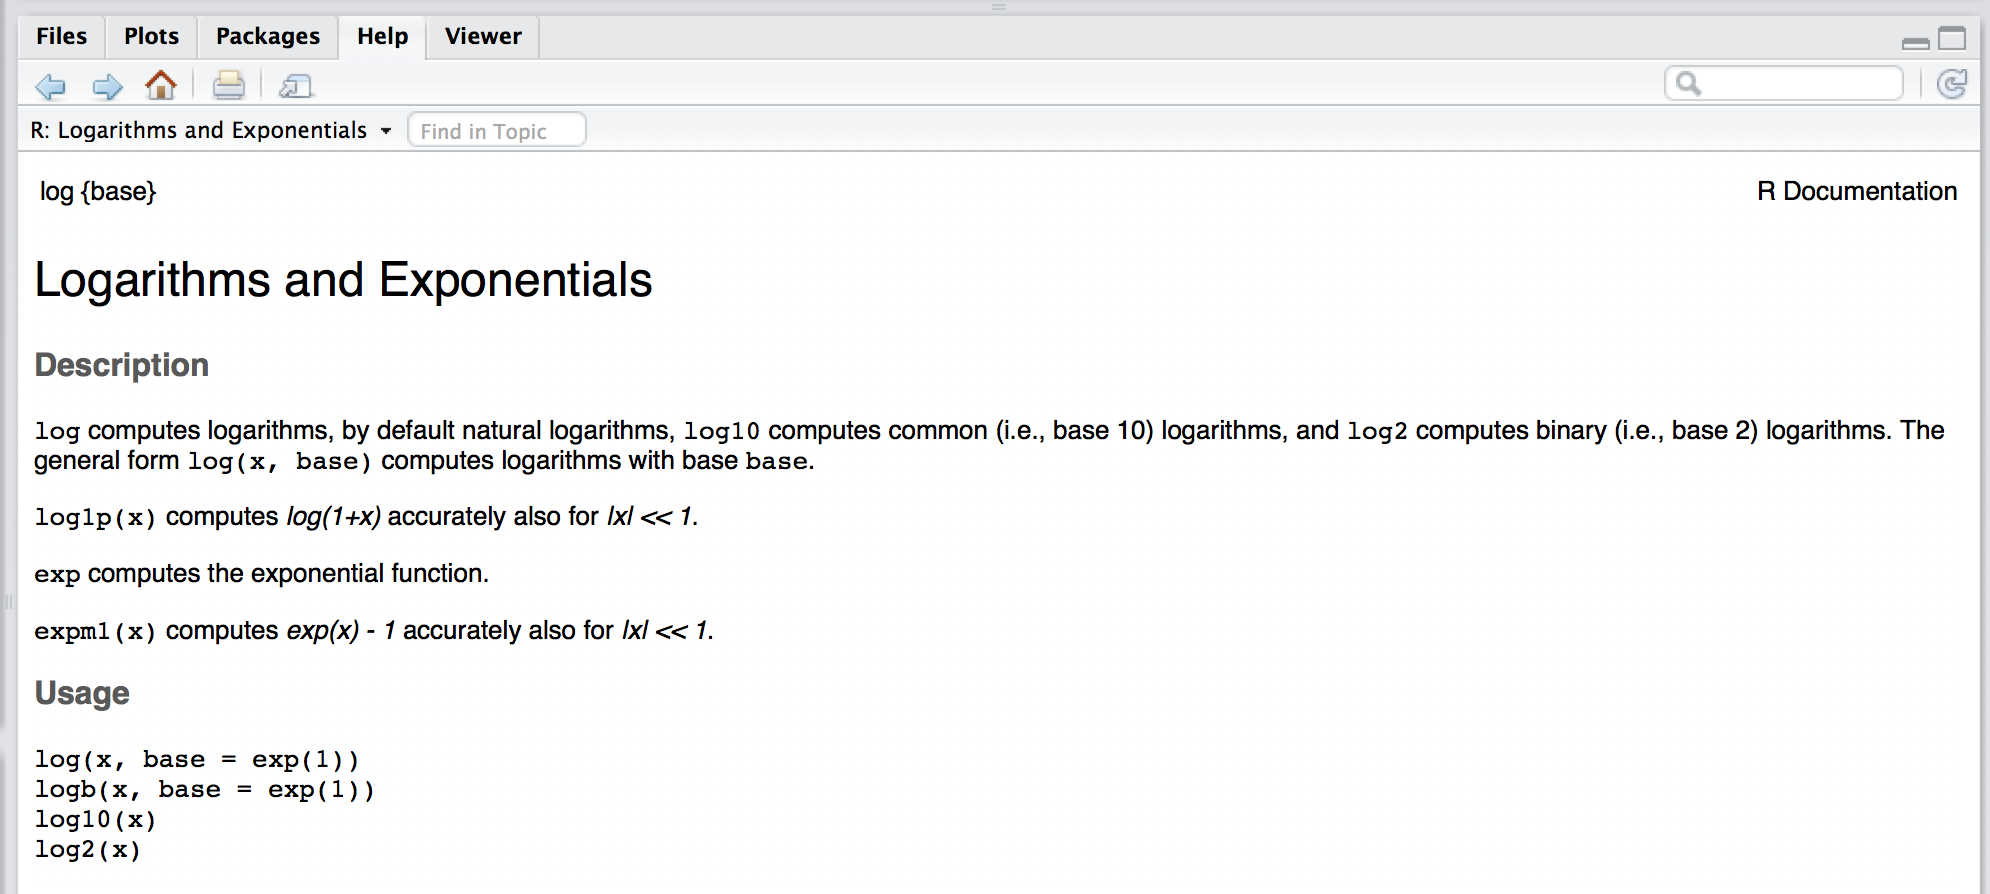
\includegraphics{images/example-log-help.png}
\caption{}
\end{figure}

The \texttt{R} documentation is written by the author of the package.
For mainstream packages in widespread use, the documentation is almost
always quite good, but in some cases it can be quite technical,
difficult to interpret, and possibly incomplete. In these cases, the
best solution to understand a function is to search for help on any
search engine. Often a simple search like ``side by side boxplots in R''
or ``side by side boxplots in ggplot2'' will produce many useful
results. The search results often include user forums such as
``CrossValidated'' or ``StackExchange'' in which the questions you have
about a function have probably already been asked and answered by many
other users.

\BeginKnitrBlock{rmdtip}
You can often use the error message to search for answers about a
problem you may have with a function.
\EndKnitrBlock{rmdtip}

\subsection{Installing packages}\label{installing-packages}

\texttt{R} comes with a number of built-in functions but one of its main
strengths is that there is a large number of packages on an
ever-increasing range of subjects available for you to install. These
packages provide additional functions, features and data to the R
environement. If you want to do something in \texttt{R} that is not
available by default, there is a good chance that there are packages
that will respond to your needs. In this case, an appropriate way to
find a package in \texttt{R} is to use the search option in the CRAN
repository which is the official network of file-transfer protocols and
web-servers that store updated versions of code and documentation for
\texttt{R} (see CRAN website). Another general approach to find a
package in \texttt{R} is simply to use a search engine in which to type
the keywords of the tools you are looking for followed by ``R package''.

\texttt{R} packages can be installed in various ways but the most widely
used approach is through the \texttt{install.packages()} function.
Another way is to use the ``Tools -\textgreater{} Install
Packages\ldots{}'' path from the dropdown menus in \texttt{RStudio} or
clicking on the ``install'' button in the ``Packages'' pane in the
RStudio environment. The \texttt{install.packages()} function is very
straight-forward and transcends any platform for the \texttt{R}
environment. It is noteworthy that this approach assumes that the
desired package(s) are available within the CRAN repository. This is
very often the case, but there is a growing number of packages that are
under-development or completed and are made available through other
repositories. In the latter setting, Chapter 02 will show other ways of
installing packages from a commonly used repository called ``GitHub''.

Sticking momentarily to the packages available in the CRAN repository,
the use of the \texttt{install.packages()} is quite simple. For example,
if you want to install the package \texttt{devtools} you can simply
write:

\begin{Shaded}
\begin{Highlighting}[]
\KeywordTok{install.packages}\NormalTok{(}\StringTok{"devtools"}\NormalTok{)}
\end{Highlighting}
\end{Shaded}

Once a package is installed it is not directly usable within your
\texttt{R} session. To do so you will have to ``load'' the package into
your current \texttt{R} session which is generally done through the
function \texttt{library()}. For example, after having installed the
\texttt{devtools} package, in order to use it within your session you
would write:

\begin{Shaded}
\begin{Highlighting}[]
\KeywordTok{library}\NormalTok{(devtools)}
\end{Highlighting}
\end{Shaded}

Once this is done, all the functions and documentation of this package
are available and can be used within your current session. However, once
you close your \texttt{R} session, all loaded packages will be closed
and you will have to load them again if you want to use them in a new
\texttt{R} session.

\BeginKnitrBlock{rmdnote}
Please notice that although packages need to be loaded at each session
if you want to use them, they need to be installed only once. The only
exception to this rule is when you need to update the package or
reinstall it for some reason.
\EndKnitrBlock{rmdnote}

One of the main packages that is required for this class would be our
STAT 297 package, that contains all the necessary packages and functions
that will be utilized in this course. Run the following code to install
the package directly from GitHub.

\begin{Shaded}
\begin{Highlighting}[]
\KeywordTok{install_github}\NormalTok{(}\StringTok{"SMAC-Group/stat297"}\NormalTok{)}
\end{Highlighting}
\end{Shaded}

\subsection{Additional References}\label{additional-references}

There are many more elements in RStudio, and we encourage you to use the
\href{https://www.rstudio.com/wp-content/uploads/2016/01/rstudio-IDE-cheatsheet.pdf}{RStudio
Cheatsheet} as a reference.

\section{\texorpdfstring{Basic Probability and Statistics with
\texttt{R}}{Basic Probability and Statistics with R}}\label{basic-probability-and-statistics-with-r}

The \texttt{R} environment provides an up-to-date and efficient
programming language to develop different tools and applications.
Nevertheless, its main functionality lies in the core statistical
framework and tools that consistute the basis of this language. Indeed,
this book aims at introducing and describing the methods and approaches
of statistical programming which therefore require a basic knowledge of
Probability and Statistics in order to grasp the logic and usefulness of
the features presented in this book.

For this reason, we will briefly take the reader through some of the
basic functions that are available within \texttt{R} to obtain
probabilities based on parametric distributions, compute summary
statistics and understand basic data structures. The latter is just an
introduction and a more in-depth description of different data
structures will be given in a future chapter.

\subsection{Probability Distributions}\label{probability-distributions}

Probability distributions can be uniquely characterized by different
functions such as, for example, their density or distribution functions.
Based on these it is possible to compute theoretical quantiles and also
randomly sample observations from them. Replacing the \texttt{R} syntax
for a given probability distribution with the general syntax
\texttt{name}, all these functions and calculations are made available
in \texttt{R} through the built-in functions:

\begin{itemize}
\tightlist
\item
  \texttt{dname} calculates the value of the density function (pdf);
\item
  \texttt{pname} calculates the value of the distribution function
  (cdf);
\item
  \texttt{qname} calculates the value of the theoretical quantile;
\item
  \texttt{rname} generates a random sample from a particular
  distribution.
\end{itemize}

Note that, when using these functions in practice, \texttt{name} is
replaced with the syntax used in \texttt{R} to denote a specific
probability distribution. For example, if we wish to deal with a Uniform
probability distribution, then the syntax \texttt{name} is replaced by
\texttt{unif} and, furthering the example, to randomly generate
observations from a uniform distribution the function to use will be
therefore \texttt{runif}. \texttt{R} allows to make use of these
functions for a wide variety of probability distributions that include,
but are not limited to: Gaussian (or Normal), Binomial, Chi-square,
Exponential, F-distribution, Geometric, Poisson, Student-t and Uniform.
In order to get an idea of how these functions can be used, below is an
example of a problem that can be solved using them.

\subsubsection{Example: Normal Test Scores of College Entrance
Exam}\label{example-normal-test-scores-of-college-entrance-exam}

Assume that the test scores of a college entrance exam follows a Normal
distribution. Furthermore, suppose that the mean test score is 70 and
that the standard deviation is 15. How would we find the percentage of
students scoring 90 or more in this exam?

In this case, we consider a random variable \(X\) that is normally
distributed as follows: \(X \sim N(\mu=70, \sigma^2=225)\) where \(\mu\)
and \(\sigma^2\) represent the mean and variance of the distribution
respectively. Since we are looking for the probability of students
scoring higher than 90, we are interested in finding
\(\mathbb{P}(X > x=90)\) and therefore we look at the upper tail of the
Normal distribution. To find this probability we need the distribution
function (\texttt{pname}) for which we therefore replace \texttt{name}
with the \texttt{R} syntax for the Normal distribution: \texttt{norm}.
The distribution function in \texttt{R} has various parameters to be
specified in order to compute a probability which, at least for the
Normal distribution, can be found by typing \texttt{?pnorm} in the
Console and are:

\begin{itemize}
\tightlist
\item
  \texttt{q}: the quantile we are interested in (e.g.~90);
\item
  \texttt{mean}: the mean of the distribution (e.g.~70);
\item
  \texttt{sd}: the standard deviation of the distribution (e.g.~15);
\item
  \texttt{lower.tail}: a boolean determining whether to compute the
  probability of being smaller than the given quantile (i.e.
  \(\mathbb{P}(X \leq x)\)) which requires the default argument
  \texttt{TRUE} or larger (i.e. \(\mathbb{P}(X > x)\)) which requires to
  specify the argument \texttt{FALSE}.
\end{itemize}

Knowing these arguments, it is now possible to compute the probability
we are interested in as follows:

\begin{Shaded}
\begin{Highlighting}[]
\KeywordTok{pnorm}\NormalTok{(}\DataTypeTok{q =} \DecValTok{90}\NormalTok{, }\DataTypeTok{mean =} \DecValTok{70}\NormalTok{, }\DataTypeTok{sd =} \DecValTok{15}\NormalTok{, }\DataTypeTok{lower.tail =} \OtherTok{FALSE}\NormalTok{) }
\end{Highlighting}
\end{Shaded}

\begin{verbatim}
## [1] 0.09121122
\end{verbatim}

As we can see from the output, there is roughly a 9\% probability of
students scoring 90 or more on the exam.

\subsection{Summary Statistics}\label{summary-statistics}

While the previous functions deal with theoretical distributions, it is
also necessary to deal with real data from which we would like to
extract information. Supposing--as is often the case in applied
statistics--we don't know from which distribution it is generated, we
would be interested in understanding the behavior of the data in order
to eventually identify a distribution and estimate its parameters.

The use of certain functions varies according to the nature of the
inputs since these can be, for example, numerical or factors.

\subsubsection{Numerical Input}\label{numerical-input}

A first step in analysing numerical inputs is given by computing summary
statistics of the data which, in this section, we can generally denote
as \texttt{x} (we will discuss the structure of this data more in detail
in the following chapters). For central tendency or spread statistics of
a numerical input, we can use the following \texttt{R} built-in
functions:

\begin{itemize}
\tightlist
\item
  \texttt{mean} calculates the mean of an input \texttt{x};
\item
  \texttt{median} calculates the median of an input \texttt{x};
\item
  \texttt{var} calculates the variance of an input \texttt{x};
\item
  \texttt{sd} calculates the standard deviation of an input \texttt{x};
\item
  \texttt{IQR} calculates the interquartile range of an input
  \texttt{x};
\item
  \texttt{min} calculates the minimum value of an input \texttt{x};
\item
  \texttt{max} calculates the maximum value of an input \texttt{x};
\item
  \texttt{range} returns a vector containing the minimum and maximum of
  all given arguments;
\item
  \texttt{summary} returns a vector containing a mixture of the above
  functions (i.e.~mean, median, first and third quartile, minimum,
  maximum).
\end{itemize}

\subsubsection{Factor Input}\label{factor-input}

If the data of interest is a factor with different categories or levels,
then different summaries are more appropriate. For example, for a factor
input we can extract counts and percentages to summarize the variable by
using \texttt{table}. Using functions and data structures that will be
described in the following chapters, below we create an example dataset
with 90 observations of three different colors: 20 being
\texttt{Yellow}, 10 being \texttt{Green} and 50 being \texttt{Blue}. We
then apply the \texttt{table} function to it:

\begin{Shaded}
\begin{Highlighting}[]
\KeywordTok{table}\NormalTok{(}\KeywordTok{as.factor}\NormalTok{(}\KeywordTok{c}\NormalTok{(}\KeywordTok{rep}\NormalTok{(}\StringTok{"Yellow"}\NormalTok{, }\DecValTok{20}\NormalTok{), }\KeywordTok{rep}\NormalTok{(}\StringTok{"Green"}\NormalTok{, }\DecValTok{10}\NormalTok{), }\KeywordTok{rep}\NormalTok{(}\StringTok{"Blue"}\NormalTok{, }\DecValTok{50}\NormalTok{))))}
\end{Highlighting}
\end{Shaded}

\begin{verbatim}
## 
##   Blue  Green Yellow 
##     50     10     20
\end{verbatim}

By doing so we obtain a frequency (count) table of the colors.

\subsubsection{Dataset Inputs}\label{dataset-inputs}

In many cases, when dealing with data we are actually dealing with
datasets (see Chapter 03) where variables of different nature are
aligned together (usually in columns). For datasets there is another
convenient way to get simple summary statistics which consists in
applying the function \texttt{summary} to the dataset itself (instead of
simply a numerical input as seen earlier).

As an example, let us explore the
\href{https://en.wikipedia.org/wiki/Iris_flower_data_set}{Iris} flower
dataset contained in the \texttt{R} built-in \texttt{datasets} package.
The data set consists of 50 samples from each of three species of Iris
(Setosa, Virginica and Versicolor). Four features were measured from
each sample consisting in the length and the width (in centimeters) of
the both sepals and petals. This dataset is widely used as an example
since it was used by Fisher to develop a linear discriminant model based
on which he intended to distinguish the three species from each other
using combinations of these four features.

Using this dataset, let us use the \texttt{summary} function on it to
output the minimum, first quartile and thrid quartile, median, mean and
maximum statistics (for the numerical variables in the dataset) and
frequency counts (for factor inputs).

\begin{Shaded}
\begin{Highlighting}[]
\KeywordTok{summary}\NormalTok{(iris)}
\end{Highlighting}
\end{Shaded}

\begin{verbatim}
##   Sepal.Length    Sepal.Width     Petal.Length    Petal.Width   
##  Min.   :4.300   Min.   :2.000   Min.   :1.000   Min.   :0.100  
##  1st Qu.:5.100   1st Qu.:2.800   1st Qu.:1.600   1st Qu.:0.300  
##  Median :5.800   Median :3.000   Median :4.350   Median :1.300  
##  Mean   :5.843   Mean   :3.057   Mean   :3.758   Mean   :1.199  
##  3rd Qu.:6.400   3rd Qu.:3.300   3rd Qu.:5.100   3rd Qu.:1.800  
##  Max.   :7.900   Max.   :4.400   Max.   :6.900   Max.   :2.500  
##        Species  
##  setosa    :50  
##  versicolor:50  
##  virginica :50  
##                 
##                 
## 
\end{verbatim}

\section{Main References}\label{main-references}

This is not the first (or the last) book that has been written
explaining and describing statistical programming in \texttt{R}. Indeed,
this can be seen as a book that brings together and reorganizes
information and material from other sources structuring and tailoring it
to a course in basic statistical programming. The main references (which
are far from being an exhaustive review of literature) that can be used
to have a more in-depth view of different aspects treated in this book
are:

\begin{itemize}
\tightlist
\item
  \citet{wickham2014advanced} : a more technical and advanced
  introduction to \texttt{R};
\item
  \citet{wickham2015packages} : basic building blocks of building
  packages in \texttt{R};
\item
  \citet{xie2015} : an overview of document generation in \texttt{R};
\end{itemize}

\section{License}\label{license}

You can redistribute it and/or modify this book under the terms of the
Creative Commons Attribution-NonCommercial-ShareAlike 4.0 International
License (CC BY-NC-SA) 4.0 License.

\chapter{RMarkdown}\label{rmarkdown}

RMarkdown is a framework that provides a literate programming format for
data science. It can be used to save and execute R code within RStudio,
and also as a simple formatting syntax for authoring HTML, PDF, ODT,
RTF, and MS Word documents as well as seamless transitions between
available formats. The name ``markdown'' is an intentional contrast to
other ``markup'' languages--e.g., hypertext markup language
(HTML)--which require syntax that can be quite difficult to decipher for
the uninitiated. One aim of the markdown paradigm is a syntax that is as
human-readable as possible. ``RMarkdown'' is an implementation of the
``markdown'' language dsigned to accommodated embedded \texttt{R} code.

What is \textbf{literate} programming?

Literate programming is the notion for programmers of adding narrative
context with code to produce documententation for the program
simultaneously. Consequently, it is possible to read through the code
with explanations so that any viewer can follow through the
presentation. RMarkdown offers a simple tool that allows to create
reports or presentation slides in a reproducible manner with collateral
advantages such as avoiding repetitive tasks by, for example, changing
all figures when data are updated.

What is \textbf{reproducible} research?

Reproducible research or reproducible analysis is the notion that an
experiment's whole process, including collecting data, performing
analysis, and producing output can be reproduced the same way by someone
else. Building non-reproducible experiments has been a problem both in
research and in the industry, and having such an issue highly decreases
the credibility of the author's findings and potentially, the author. In
essence, allowing for reproducible research implies that anyone could
run the code (knit the document, etc.) and obtain the same exact results
as the original research and RMarkdown is commonly used to address this
issue.

\section{Initialize and create an R Markdown file in
RStudio}\label{initialize-and-create-an-r-markdown-file-in-rstudio}

Within RStudio, click \texttt{File} → \texttt{New\ File} →
\texttt{R\ Markdown}. Give the file\footnote{\url{http://kbroman.org/datacarpentry_R_2017-01-10/img/New_R_Markdown.png}}
a title and the author (your name) and select the default output, HTML.
We can change this later so don't worry about it.

\begin{figure}[htbp]
\centering
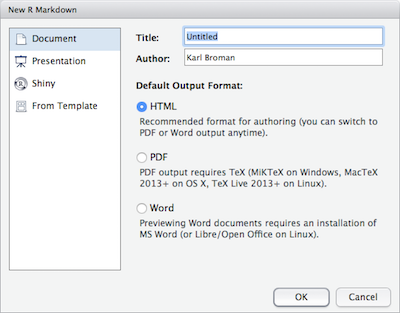
\includegraphics{images/rmd_new.png}
\caption{}
\end{figure}

An RMarkdown is a plain text file that contains three different aspects:

\begin{itemize}
\tightlist
\item
  YAML metadata
\item
  Code Chunks
\item
  Text
\end{itemize}

\section{YAML Metadata}\label{yaml-metadata}

YAML stands for \emph{YAML Ain't Markup Language}, and is used to
specify document configurations and properties such as name, date,
output format, etc. The (optional) YAML header surrounded before and
after by ``---'' on a dedicated line.

\begin{figure}[htbp]
\centering
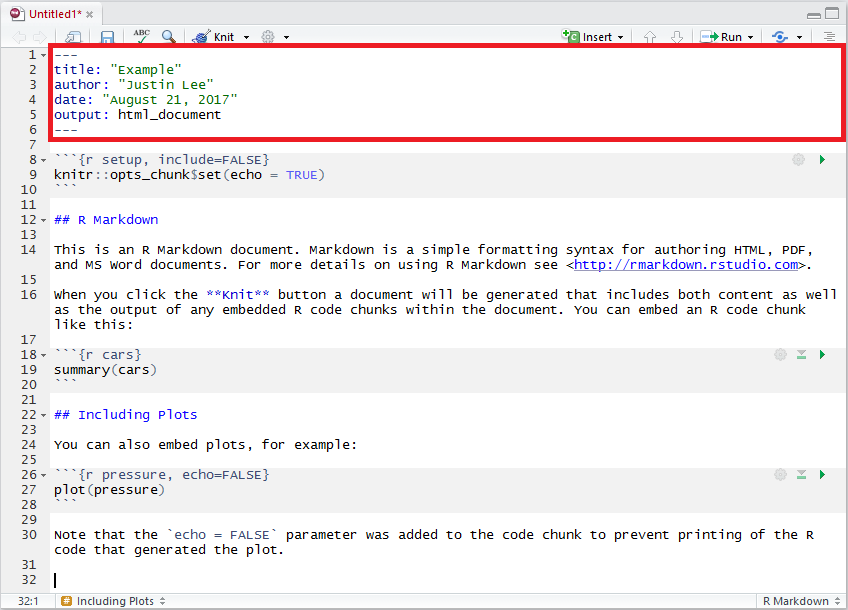
\includegraphics{images/rmd_yaml.png}
\caption{}
\end{figure}

You can also include additional formatting
\href{http://rmarkdown.rstudio.com/html_document_format.html}{options},
such as a table of contents, or even a custom CSS style template which
can utilized to further enhance presentation. For the purpose of the
class, the default options should be sufficient. Below is an example
knit output of the above RMarkdown file.

\begin{figure}[htbp]
\centering
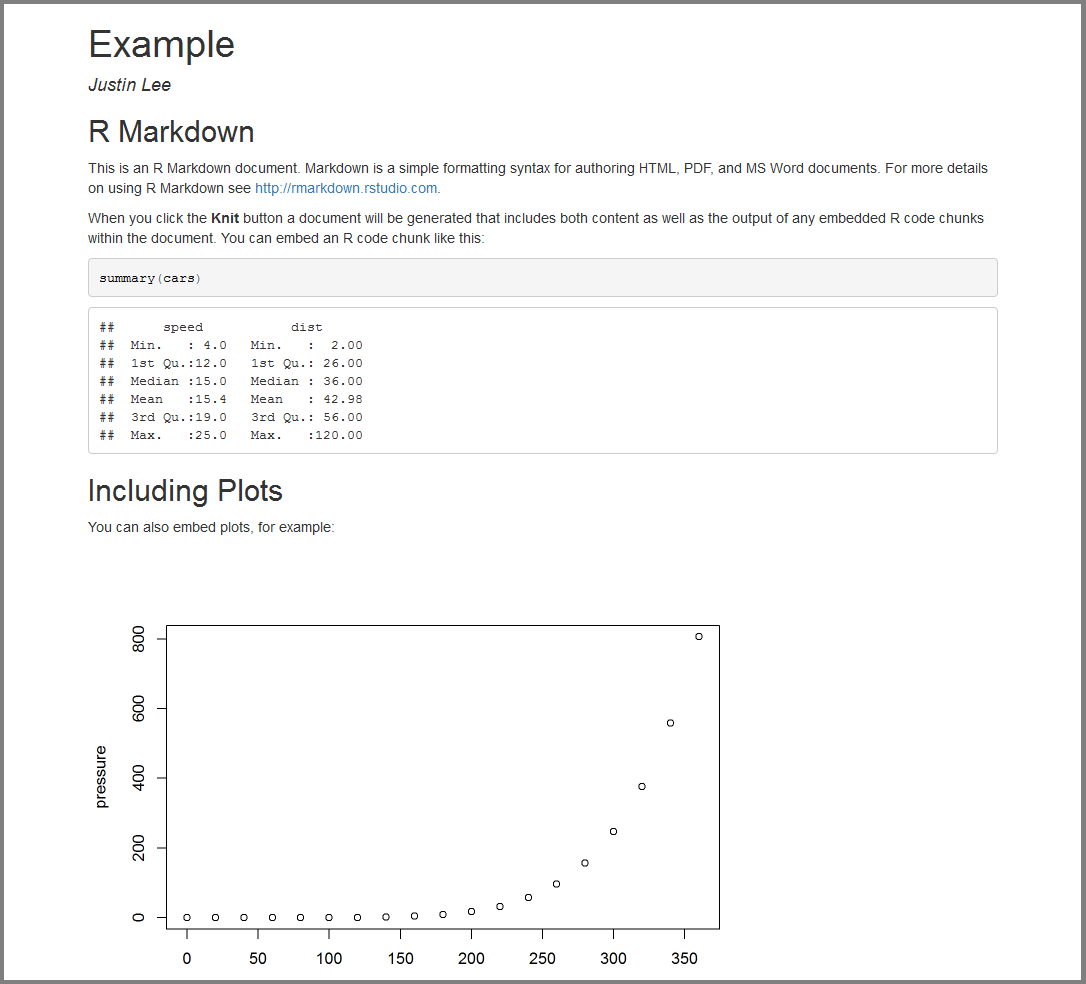
\includegraphics{images/rmd_example_output.png}
\caption{}
\end{figure}

The default output above is an html\_document format. However, this can
be specified as well, such as \texttt{pdf\_document}. The pdf format,
however, requires additional installation and configuration of a TeX
distribution such as \href{https://miktex.org/2.9/setup}{MikTeX}. Once
available, the user can also include raw LaTeX and even define LaTeX
macros in the RMarkdown document if necessary.

\subsection{Subsections}\label{subsections}

To make your sections numbered as sections and subsections, make sure
you specify \texttt{number\_sections:\ yes} as part of the YAML Metadata
as shown below.

\begin{figure}[htbp]
\centering
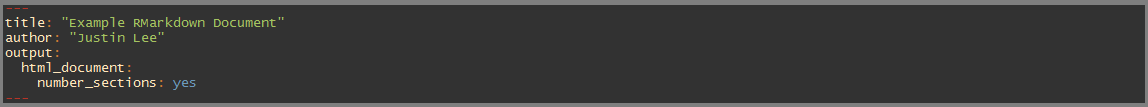
\includegraphics{images/yaml_number_sections.png}
\caption{}
\end{figure}

\section{Text}\label{text}

In addition, due to its literate nature, text will be an essential part
in explaining your analysis. With RMarkdown, we can specify custom text
formatting, such as with emphasis such as \emph{italics}, \textbf{bold},
or \texttt{code\ style}. To understand how to format text, our previous
would be as follows in RMarkdown:

\begin{verbatim}
With RMarkdown, we can specify custom text formatting, such as with emphasis such as *italics*, **bold**, or even a `code style`.
\end{verbatim}

\begin{figure}[htbp]
\centering
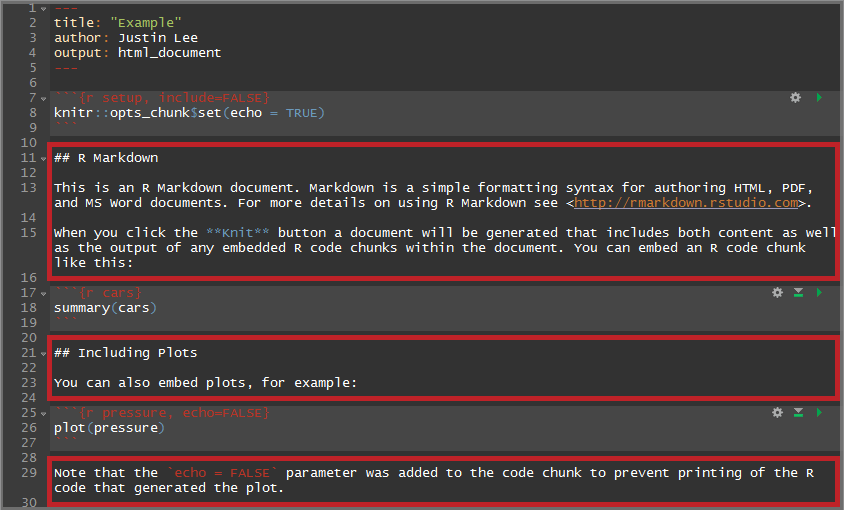
\includegraphics{images/rmd_text.png}
\caption{}
\end{figure}

\subsection{Headers}\label{headers}

As seen above, headings are preceded with a \#. A single \texttt{\#}
produces the largest heading text; to output smaller headings, simply
add more \#! Heading level also impacts section and subsection nesting
in documents and tables of contents, as well as slide breaks in
presentation formats.

\subsection{Lists}\label{lists}

Lists can be extremely convienient to make text more readable or to take
course notes during class. RMarkdown allows to create different list
structures as shown in the code below:

\begin{verbatim}
* You can create bullet points by using symbols such as *, +, or -. 
+ simply add an indent or four preceding spaces to indent a list. 
    + You can manipulate the number of spaces or indents to your liking. 
        - Like this. 
    * Here we go back to the first indent. 
1. To make the list ordered, use numbers. 
1. We can use one again to continue our ordered list. 
2. Or we can add the next consecutive number. 
\end{verbatim}

which delivers the following list structure:

\begin{itemize}
\tightlist
\item
  You can create bullet points by using symbols such as *, +, or -.
\item
  Simply add an indent or four preceding spaces to indent a list.

  \begin{itemize}
  \tightlist
  \item
    You can manipulate the number of spaces or indents to your liking.

    \begin{itemize}
    \tightlist
    \item
      Like this.
    \end{itemize}
  \item
    Here we go back to the first indent.
  \end{itemize}
\end{itemize}

\begin{enumerate}
\def\labelenumi{\arabic{enumi}.}
\tightlist
\item
  To make the list ordered, use numbers instead of symbols.
\item
  Here we write the next consecutive number to continue.

  \begin{itemize}
  \tightlist
  \item
    Add more content by indenting like before.
  \end{itemize}
\end{enumerate}

\subsection{Hyperlinks}\label{hyperlinks}

To add hyperlinks with the full link, (ex: \url{https://google.com/})
you can follow the syntax below:

\begin{verbatim}
<https://google.com/>
\end{verbatim}

whereas to add hyperlinks with a custom link title, (ex:
\href{https://google.com}{Google}) follow the syntax below:

\begin{verbatim}
[Google](https://google.com)
\end{verbatim}

\subsection{Blockquotes}\label{blockquotes}

\textbf{Same thing for citation\ldots{} What do you think?}

\begin{quote}
Use the \textgreater{} character in front of a line, \emph{just like in
email}. Use it if you're quoting a person, a song or whatever.
\end{quote}

\subsection{Pictures}\label{pictures}

To add a picture with captions, follow the syntax below:

\begin{verbatim}
![Eberly College of Science Banner](http://science.psu.edu/psu_eberly_blue.png)
\end{verbatim}

\begin{figure}[htbp]
\centering

\includegraphics{http://science.psu.edu/psu_eberly_blue.png}
\caption{Eberly College of Science Banner}
\end{figure}

Else, to add a picture without any captions, follow the syntax below:

\begin{verbatim}
![](http://kefalosandassociates.com/wp-content/uploads/2015/07/facebook-banner.png)
\end{verbatim}

\begin{figure}[htbp]
\centering
\includegraphics{http://kefalosandassociates.com/wp-content/uploads/2015/07/facebook-banner.png}
\caption{}
\end{figure}

\subsection{LaTeX}\label{latex}

What is \textbf{LaTeX}?

LaTeX is a document preparation system that uses plain text as opposed
to formatted text used for applications such as Microsoft Word. It is
widely used in academia as a standard for the publication of scientific
documents. It has control over large documents containing sectioning,
cross-references, tables and figures.

\subsubsection{LaTeX in RMarkdown}\label{latex-in-rmarkdown}

Unlike a highly formatted word processor, we cannot produce equations by
clicking on symbols. As data scientists we need to explain distributions
and equations that are behind the methods we present. Within the text
section of an RMarkdown document you can include LaTeX format text to
output different forms of text, mainly equations and mathematical
expressions.

Inline mathematical expressions can be added using the syntax:
\texttt{\$math\ expression\$}. For example, if we want to write ``where
\(\alpha\) is in degrees'' we would write:

\begin{verbatim}
"where $\alpha$ is in degrees".
\end{verbatim}

Using a slightly different syntax (i.e.
\texttt{\$\$math\ expression\$\$}) we can obtain centered mathematical
expressions. For example, the binomial probability in LaTeX is written
as

\texttt{\$\$f(y\textbar{}N,p)\ =\ \textbackslash{}frac\{N!\}\{y!(N-y)!\}\textbackslash{}cdot\ p\^{}y\ \textbackslash{}cdot\ (1-p)\^{}\{N-y\}\ =\ \{\{N\}\textbackslash{}choose\{y\}\}\ \textbackslash{}cdot\ p\^{}y\ \textbackslash{}cdot\ (1-p)\^{}\{N-y\}\$\$}

which is output as:

\[f(y|N,p) = \frac{N!}{y!(N-y)!}\cdot p^y \cdot (1-p)^{N-y} = {{N}\choose{y}} \cdot p^y \cdot (1-p)^{N-y}\]

An introduction to the LaTeX format can be found
\href{http://www.math.harvard.edu/texman/}{here} if you want to learn
more about the basics. An alternative can be to insert custom LaTeX
formulas using a graphical interface such as
\href{https://www.codecogs.com/latex/eqneditor.php}{codecogs}.

\subsection{Cross-referencing
Sections}\label{cross-referencing-sections}

You can also use the same syntax \texttt{\textbackslash{}@ref(label)} to
reference sections, where label is the section identifier (ID). By
default, Pandoc will generate IDs for all section headers, e.g.,
\texttt{\#\ Hello\ World} will have an ID \texttt{hello-world}. To call
header \texttt{hello-world} as a header, we type
\texttt{\textbackslash{}@ref(hello-world)} to cross-reference the
section. In order to avoid forgetting to update the reference label
after you change the section header, you may also manually assign an ID
to a section header by appending \{\#id\} to it.

\subsection{Citations and
Bibliography}\label{citations-and-bibliography}

Citations and bibliographies can automatically be generated with
RMarkdown. In order to use this feature we first need to create a
``BibTex'' database which is a simple plain text file (with the
extension ``.bib'') where each reference you would like to cite is
entered in a specific manner.

To illustrate how this is done, let us take the example of a recent
paper where two researchers from Oxford University investigated the
connection between the taste of food and various features of cutlery
such as weight and colour (calling this phenomenon the ``taste of
cutlery''). The bibtex ``entry'' for this paper is given below:

\begin{verbatim}
@article{harrar2013taste,
  title={The taste of cutlery: how the taste of food is affected by the weight, size,
   shape, and colour of the cutlery used to eat it},
  author={Harrar, Vanessa and Spence, Charles},
  journal={Flavour},
  volume={2},
  number={1},
  pages={21},
  year={2013},
  publisher={BioMed Central}
}
\end{verbatim}

This may look like a complicated format to save a reference but there is
an easy way to obtain this format without having to manually fill in the
different slots. To do so, go online and search for ``Google Scholar''
which is a search engine specifically dedicated to academic or other
types of publications. In the latter search engine you can insert
keywords or the title and/or authors of the publication you are
interested in and find it in the list of results. In our example we
search for ``The tast of cutlery'' and the publication we are interested
in is the first in the results list.

\begin{figure}[htbp]
\centering
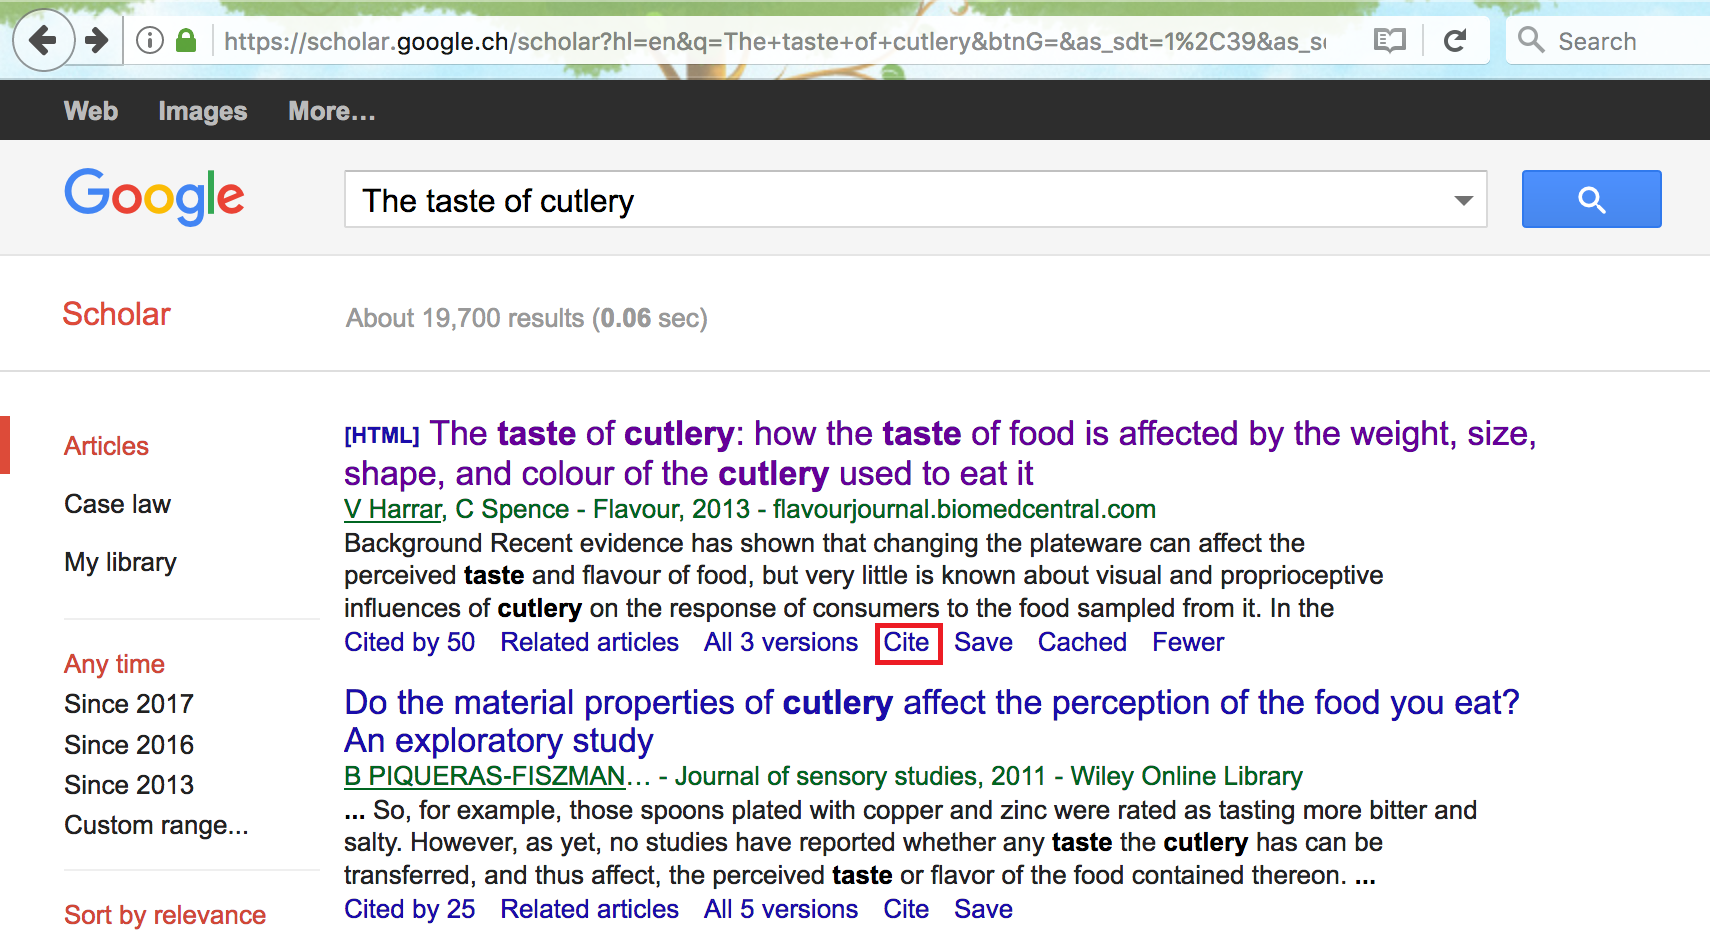
\includegraphics{images/googlescholar1.png}
\caption{}
\end{figure}

Below every publication in the list there is a set of options among
which the one we are interested in is the ``Cite'' option that should
open a window in which a series of reference options are available.
Aside from different reference formats that can be copied and pasted
into your document, at the bottom of the window you can find another set
of options (with related links) that refer to different bibliography
managers.

\begin{figure}[htbp]
\centering
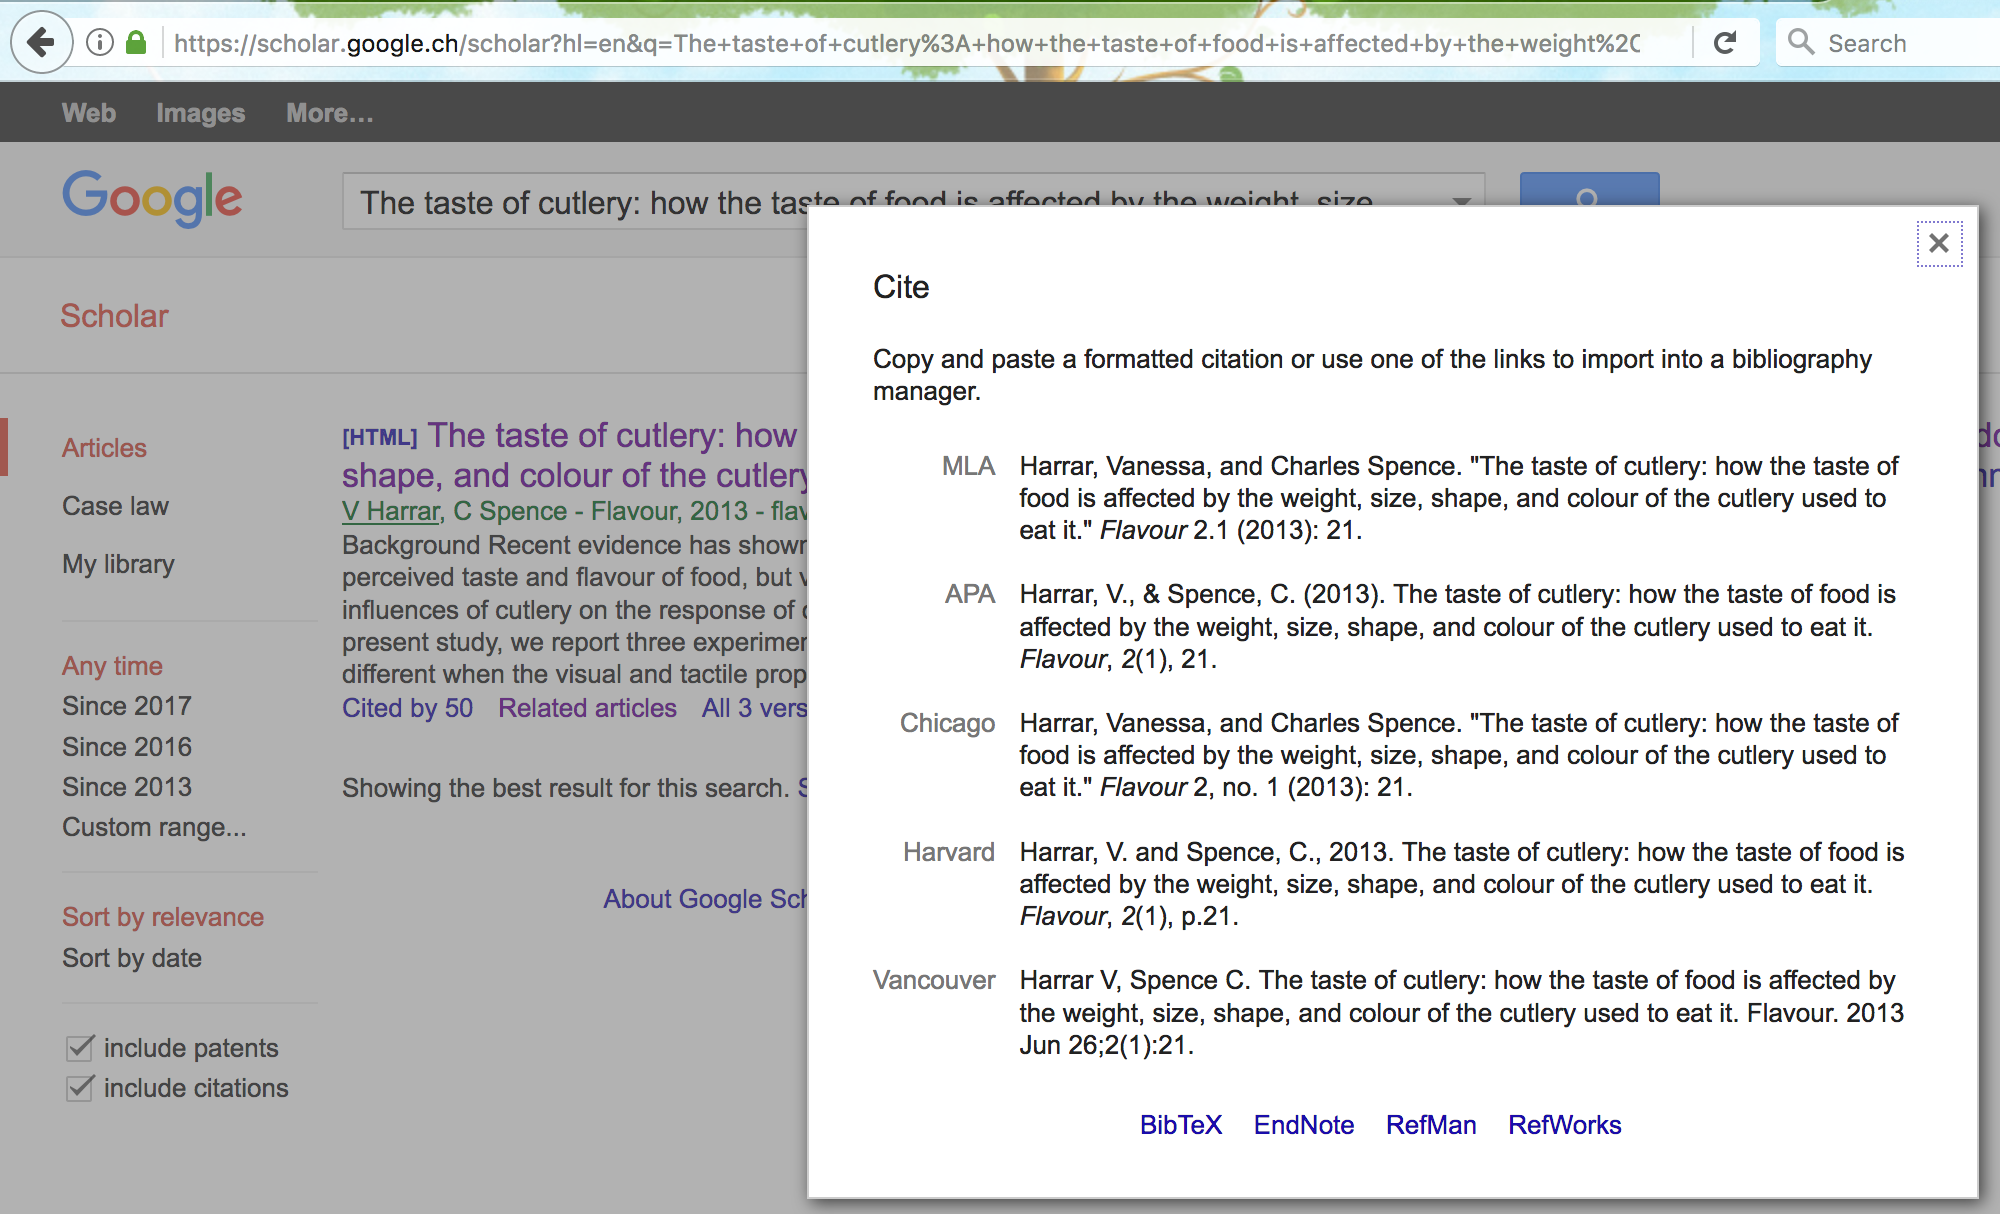
\includegraphics{images/googlescholar2.png}
\caption{}
\end{figure}

For ``.bib'' files we are interested in the ``BibTex'' option and by
clicking on it we will be taken to another tab in which the format of
the reference we want is provided. All that needs to be done at this
point is to copy this format (that we saw earlier in this section) and
paste in the ``.bib'' file you created and save the changes.

\begin{figure}[htbp]
\centering
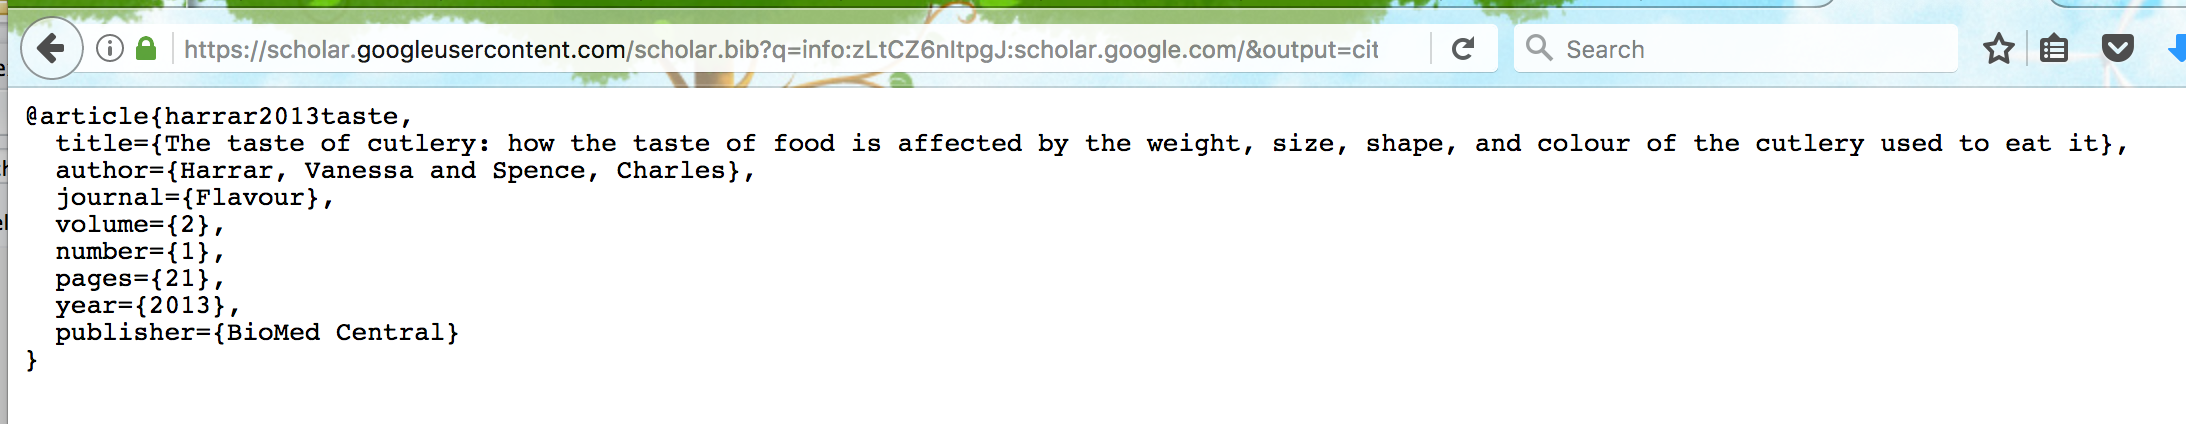
\includegraphics{images/googlescholar3.png}
\caption{}
\end{figure}

However, your Rmarkdown document does not know about the existence of
this bibliography file and therefore we need to insert this information
in the YAML metadata at the start of our document. To do so, let us
suppose that you named this file ``biblio.bib'' (saved in the same
location as your Rmarkdown document). All that needs to be done is to
add another line in the YAML metadata with
\texttt{bibliography:\ biblio.bib} and your Rmarkdown will now be able
to recognise the references within your ``.bib'' file. There are also a
series of other options that can be specified for the bibliography such
as its format or the way references can be used within the text (for a
more detailed overview the BibTex environment and managing references in
Rmarkdown see, for example, this
\href{https://www.economics.utoronto.ca/osborne/latex/BIBTEX.HTM}{link}
and this
\href{http://rmarkdown.rstudio.com/authoring_bibliographies_and_citations.html}{link}
respectively).

Once the ``.bib'' file has been created and has been linked to your
Rmarkdown document through the details in the YAML metadata, you can now
start using the references you have collected in the ``.bib'' file. To
insert these references within your document at any point of your text
you need to use the name that starts the reference field in your
``.bib'' file and place it immediately after the \texttt{@} symbol
(without spaces). So, for example, say that we wanted to cite the
publication on the ``taste of cutlery'': in your Rmarkdown all you have
to do is to type \texttt{@harrar2013taste} at the point where you want
this citation in the text and you will obtain: \citet{harrar2013taste}.

\BeginKnitrBlock{rmdnote}
The user can also change the name that is used to call the desired
reference as long as the same name is used to cite it in the Rmarkdown
document and that this name is not the same as another reference.
\EndKnitrBlock{rmdnote}

\BeginKnitrBlock{rmdcaution}
The references in the ``.bib'' file will not appear in the references
that are output from the Rmarkdown compiling procedure unless they are
specifically used within the Rmarkdown document.
\EndKnitrBlock{rmdcaution}

Additional References:

\begin{itemize}
\tightlist
\item
  \href{https://www.economics.utoronto.ca/osborne/latex/BIBTEX.HTM}{Intro
  to bibtex}
\item
  \href{http://rmarkdown.rstudio.com/authoring_bibliographies_and_citations.html}{Ref
  on ref for rmd}
\end{itemize}

\subsection{Tables}\label{tables}

For simple tables, we can be manually insert values as such,

\begin{verbatim}
+---------------+---------------+--------------------+
| Fruit         | Price         | Advantages         |
+===============+===============+====================+
| *Bananas*     | $1.34         | - built-in wrapper |
|               |               | - bright color     |
+---------------+---------------+--------------------+
| Oranges       | $2.10         | - cures scurvy     |
|               |               | - **tasty**        |
+---------------+---------------+--------------------+
\end{verbatim}

to produce:

\begin{longtable}[]{@{}lll@{}}
\toprule
\begin{minipage}[b]{0.20\columnwidth}\raggedright\strut
Fruit\strut
\end{minipage} & \begin{minipage}[b]{0.20\columnwidth}\raggedright\strut
Price\strut
\end{minipage} & \begin{minipage}[b]{0.27\columnwidth}\raggedright\strut
Advantages\strut
\end{minipage}\tabularnewline
\midrule
\endhead
\begin{minipage}[t]{0.20\columnwidth}\raggedright\strut
\emph{Bananas}\strut
\end{minipage} & \begin{minipage}[t]{0.20\columnwidth}\raggedright\strut
\$1.34\strut
\end{minipage} & \begin{minipage}[t]{0.27\columnwidth}\raggedright\strut
\begin{itemize}
\tightlist
\item
  built-in wrapper
\item
  bright color
\end{itemize}\strut
\end{minipage}\tabularnewline
\begin{minipage}[t]{0.20\columnwidth}\raggedright\strut
Oranges\strut
\end{minipage} & \begin{minipage}[t]{0.20\columnwidth}\raggedright\strut
\$2.10\strut
\end{minipage} & \begin{minipage}[t]{0.27\columnwidth}\raggedright\strut
\begin{itemize}
\tightlist
\item
  cures scurvy
\item
  \textbf{tasty}
\end{itemize}\strut
\end{minipage}\tabularnewline
\bottomrule
\end{longtable}

As an alternative we can use the simple graphical user interface
\href{http://www.tablesgenerator.com/markdown_tables}{online}. For more
extensive tables, we create dataframe objects and project them using
\texttt{knitr::kable()}, which we will explain later.

\subsection{Additional References}\label{additional-references-1}

There are many more elements to creating a useful report using
RMarkdown, and we encourage you to use the
\href{https://www.rstudio.com/wp-content/uploads/2015/02/rmarkdown-cheatsheet.pdf}{Rmarkdown
Cheatsheet} as a reference.

\section{Code Chunks}\label{code-chunks}

This is where you enter your code.

You can quickly insert chunks like these into your file with

\begin{itemize}
\tightlist
\item
  the keyboard shortcut Ctrl + Alt + I (OS X: Cmd + Option + I)
\item
  the Add Chunk command in the editor toolbar
\item
  by typing the chunk delimiters \textbf{```\{\r\}} and \textbf{```}.
\end{itemize}

\begin{figure}[htbp]
\centering
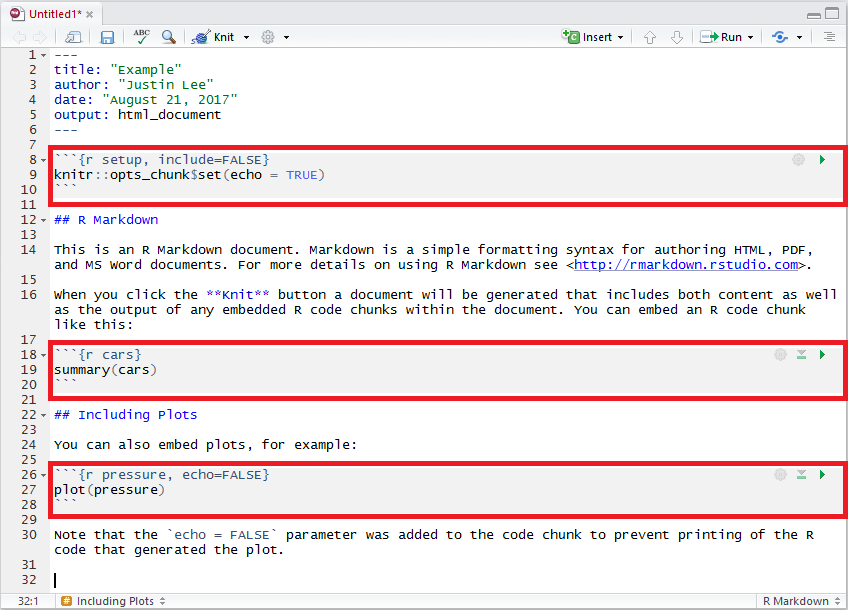
\includegraphics{images/rmd_code_chunk.png}
\caption{}
\end{figure}

\subsection{Code Chunk Options}\label{code-chunk-options}

In the third code chunk above, we also configure chunk options. Note
that the \texttt{echo\ =\ FALSE} parameter was added to the code chunk
to prevent printing of the R code that generated the plot. This is a
useful way to embed figures. More options can be referred from the
\href{https://www.rstudio.com/wp-content/uploads/2015/02/rmarkdown-cheatsheet.pdf}{Rmarkdown
Cheatsheet} and Yihui's notes on knitr
\href{https://yihui.name/knitr/options/}{options}. Here are some
explanations of the most commonly used chunk options exerted from above:

\begin{itemize}
\tightlist
\item
  eval: (TRUE; logical) whether to evaluate the code chunk
\item
  echo: (TRUE; logical or numeric) whether to include R source code in
  the output file
\item
  warning: (TRUE; logical) whether to preserve warnings (produced by
  warning()) in the output like we run R code in a terminal (if FALSE,
  all warnings will be printed in the console instead of the output
  document)
\item
  cache: (FALSE; logical) whether to cache a code chunk;
\end{itemize}

Plot figure options:

\begin{itemize}
\tightlist
\item
  fig.path: (`figure/'; character) prefix to be used for figure
  filenames (fig.path and chunk labels are concatenated to make
  filenames)
\item
  fig.show: (`asis'; character) how to show/arrange the plots
\item
  fig.width, fig.height: (both are 7; numeric) width and height of the
  plot, to be used in the graphics device (in inches) and have to be
  numeric
\item
  fig.align: (`default'; character) alignment of figures in the output
  document (possible values are left, right and center
\item
  fig.cap: (NULL; character) figure caption to be used in a figure
  environment
\end{itemize}

\subsection*{In-line R}\label{in-line-r}
\addcontentsline{toc}{subsection}{In-line R}

The variables we store in a RMarkdown will stay within the environment.
This means that we can call and manipulate them anywhere within the
document. In Rmarkdown, we can reference the variable in-line in the
text section by using \texttt{r\ variable} to show the value of our
variable embedded within the sentence. Here is an example:

\begin{Shaded}
\begin{Highlighting}[]
\NormalTok{a =}\StringTok{ }\DecValTok{2}
\end{Highlighting}
\end{Shaded}

Above, we stored the value 2 into \texttt{a}.

\begin{verbatim}
The value of $a$ is `r a`. 
\end{verbatim}

This translates in R Markdown to ``The value of \(a\) is 2.''

\subsection*{Cache}\label{cache}
\addcontentsline{toc}{subsection}{Cache}

Depending on the complexity of calculations in your embedded R code, it
may be convenient to avoid re-running the computations (which could be
lengthy) each time you knit the document together. For this purpose, it
possible to specify an additional argument for your embedded R code
which is the \texttt{cache} argument. By default this argument is
assigned the value \texttt{FALSE} and therefore the R code is run every
time your document is compiled. However, if you specify this argument as
\texttt{cache\ =\ TRUE}, then the code is only run the first time the
document is compiled while the following times it simply stores and
presents the results of the computations when the document was first
compiled.

Let us consider an example where we want to embed an R code with a very
simple operation such as assigning the value of 2 to an object that we
call \texttt{a} (that we saw earlier). This is clearly not the best
example since this operation runs extremely quickly and there is no
visible loss in document compilation time. However, we will use it just
to highlight how the \texttt{cache} argument works. Therefore, if we
want to avoid running this operation each time the document is compiled,
then we just embed our R code as follows:

\begin{verbatim}
a = 2
\end{verbatim}

You will notice that we called this chunk of embedded R code
\texttt{computeA} and the reason for this will become apparent further
on. Once we have done this we can compile the document that will run
this operation and store its result. Now, if we compile the document
again (independently from whether we made changes to the rest of the
document or not) this operation will not be run and the result of the
previous (first) compiling will be presented. However, if changes are
made to the R code which has been ``cached'', then the code will be run
again and this time its new result will be stored for all the following
compilings until it is changed again.

This argument can therefore be very useful when computationally
intensive R code is embedded within your document. Nevertheless it can
suffer from a drawback which consists in dependencies of your ``cached''
R code with other chunks within the document. In this case, the other
chunks of R code can be modified thereby outputting different results
but these will not be considered by your ``cached'' R code. As an
example, suppose we have another chunk of R code that we can ``cache''
and that takes the value of \texttt{a} from the previous chunk:

\begin{verbatim}
(d = 2*a)
\end{verbatim}

\begin{verbatim}
## [1] 4
\end{verbatim}

In this case, the output of this chunk will be \texttt{\#\#\ 4} since
\texttt{a\ =\ 2} (from the previous chunk). What happens however if we
modify the value of \texttt{a} in the previous chunk? In this case, the
previous chunk will be recomputed but the value of \texttt{d} (in the
following chunk) will not be updated since it has stored the value of 4
and it is not recomputed since this chunk has not been modified. To
avoid this, a solution is to specify the chunks of code that the
``cached'' code depends on. This is why we initially gave a name to the
first chunk of code (``computeA'') so as to refer to it in following
chunks of ``cached'' code that depend on it. To refer to this code you
need to use the option \texttt{dependson} as follows:

\begin{verbatim}
d = 2*a
\end{verbatim}

In this manner, if the value of \texttt{a} changes in the first chunk,
the value of \texttt{d} will also change but will be stored until either
the \texttt{computeA} chunk or the latter chunk is modified.

\section{Render Output}\label{render-output}

After you are done, run \texttt{rmarkdown::render()} or click the
\texttt{Knit} button at the top of the RStudio scripts pane to save the
output in your working directory.

\begin{figure}[htbp]
\centering
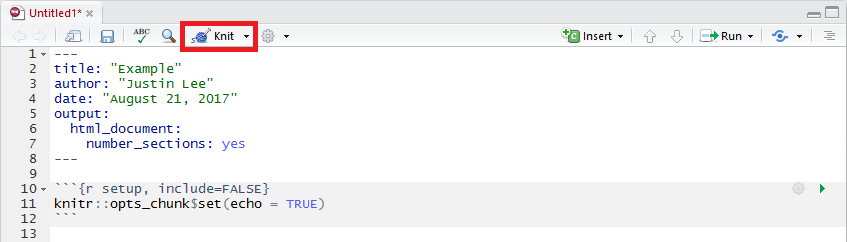
\includegraphics{images/rmd_knit.png}
\caption{}
\end{figure}

The use of RMarkdown makes it possible to generate any file format such
as HTML, pdf, and Word processor formats using \texttt{pandoc}. Pandoc
is free software understands and converts useful markdown syntax such as
code mentioned above into readable, clean format.

Click on the links below for more information on RMarkdown:

\begin{itemize}
\tightlist
\item
  \href{http://rmarkdown.rstudio.com/authoring_quick_tour.html}{RStudio
  RMarkdown tutorial}
\item
  \href{https://www.r-bloggers.com/r-markdown-and-knitr-tutorial-part-1/}{R-blogger's
  RMarkdown tutorial}
\end{itemize}

\bibliography{packages.bib,book.bib}


\end{document}
